\chapter{Research Methodology}\label{ch:research-methodology}
%\lipsum[2-8]
\initial{F}rom the literature there is a clear lack of results for localisation systems using the commercial Pozyx sensor network with drones in an household environment.
To address the aims and objectives stated in ~\ref{sec:aims_objs}, it is proposed that a lightweight on-board localisation be developed to check the feasibility of minimal hardware solution for an indoor drone.
This would entail connecting a Pozyx tag directly to a FCU and integrate it with the pose localisation system existing already.
To close the loop the pose information should be available in some format that can be used for autonomous control.
Furthermore, the system should be tested in a practical environment, to this end, the Pozyx anchor network was setup in a kitchen.
A kitchen represents one of the highest traffic areas in a household and it contains various materials that will make raw readings from a UWB system noisy and inaccurate.
As a kitchen will contain both dynamic and static obstacles multiple anchor configurations must be tested in order to find optimal anchor positions in this given environment.

\section{Anchor Configurations}\label{sec:anchor-configurations}
Noting work from ~\citet{di2019evaluation} and the setup procedures from ~\citet{pozyx2018pozyx} it is important to have at least 4 anchors setup in non-planar orientations for the best positioning results.
To determine a suitable anchor configuration in the given space a tag was placed at fixed known point in a given reference frame and the mounted locations of the 4 anchors were varied on each wall of the kitchen in order to prevent planar configurations and ambiguity when the tag calculates its position.
Figure ~\ref{fig:layout} shows a simplified layout and toybox configuration of the tag and anchors.
Grey areas represent areas in the space that is impossible to traverse, red represents known obstacles that interfere and attenuate the UWB signal, blue represent anchors, green the tag, cream is partially obstructed and the rest of the area is fully traversable.
Before each run and data collection the tag was manually configured with the location of each of the anchors in the reference frame of the kitchen and recorded for at least 5 seconds.
The tag was triggered to calculate the position repeatedly within the timeframe and the function call is blocking and takes $\approx70ms$ so data was recorded at a frequency of $\approx14.28Hz$.
With a tag position of (1480,2330,980)mm, the following statistics were calculated using Matlab.
In addition to the average error and standard deviation,  kurtosis and skew metrics were added to show the number of outliers and symmetry of the recorded data.
The error metrics are important to give an idea of how noisy the overall data is while kurtosis and skewness gives an indication if the noise follows a uniform distribution which would be beneficial ideal for state estimators.
From table ~\ref{tb:config_stats} we can see that configuration 12 gives acceptable error metrics and reasonable skew and kurtosis making it the best out of the configurations tested.
To further support this Figure ~\ref{fig:config} shows several results obtained with several configurations and it can be seen that configuration 12 produced the best results.

\begin{figure}[h!]
    \centering
    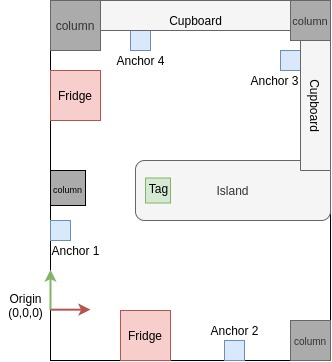
\includegraphics{mtd/Kitchen_layout}
    \caption{Birds eye view of the test environment.}
    \label{fig:layout}
\end{figure}
\newpage
%\begin{table}[h!]
   \begin{longtable}[h!]{| c | c | c | c | c | c |}
       \hline
       Config \#& Anchor positions (mm)
       & Avg. Error & Std. Deviation$\left(\begin{array}{c}
       x,\\y,\\z
       \end{array}\right)$ & Kurtosis & Skewness\\
       \hline
       1 & $\left(\begin{array}{c}
       (0,0,1115),\\(3680, -405, 1550),\\(3655, 4080, 1906),\\(270, 4465, 2090)
       \end{array}\right)$& 342.5906 & $\left(\begin{array}{c}
       183.1707,\\205.3426,\\972.6239
       \end{array}\right)$&$\left( \begin{array}{c}
       2.349,\\ 1.5967,\\ 1.415
       \end{array} \right)$&$\left( \begin{array}{c}
       -0.4083,\\ -0.3522,\\ 0.4551
       \end{array} \right)$\\
       \hline
              2 & $\left(\begin{array}{c}
       (0,665,1115),\\(2995, -405, 1889),\\(3655, 4080, 1906),\\(270, 4465, 2090)
       \end{array}\right)$& 173.5938 & $\left(\begin{array}{c}
       43.2345,\\45.6897,\\133.8616\\
       \end{array}\right)$&$\left( \begin{array}{c}
       21.8923,\\ 10.1765,\\ 119.1344
       \end{array} \right)$&$\left( \begin{array}{c}
       -2.8672,\\ -0.3453,\\ 8.9025
       \end{array} \right)$\\
       \hline
              3 & $\left(\begin{array}{c}
       (0,665,1115),\\(2995, -405, 1889),\\(3655, 4080, 1906),\\(1526, 4559, 837)
       \end{array}\right)$& 203.8502 & $\left(\begin{array}{c}
       128.4693,\\118.3216,\\209.1637
       \end{array}\right)$&$\left( \begin{array}{c}
       14.2955,\\ 11.2045,\\ 2.9124
       \end{array} \right)$&$\left( \begin{array}{c}
       -2.579,\\  -0.3920,\\ 0.4055
       \end{array} \right)$\\
       \hline
              4 & $\left(\begin{array}{c}
       (0,665,1115),\\(2995, -405, 1889),\\(3655, 4080, 1906),\\(1070, 5170, 491)
       \end{array}\right)$& 85.8562 & $\left(\begin{array}{c}
       40.2197,\\40.6081,\\66.2120
       \end{array}\right)$&$\left( \begin{array}{c}
       6.7558,\\ 7.5180,\\ 3.4722
       \end{array} \right)$&$\left( \begin{array}{c}
       -0.4260,\\ -0.5344,\\ -0.1242
       \end{array} \right)$\\
       \hline
              5 & $\left(\begin{array}{c}
       (0,665,1115),\\(2995, -405, 1889),\\(3960, 3368, 2304),\\(1070, 5170, 491)
       \end{array}\right)$& 64.8616 & $\left(\begin{array}{c}
       65.3883,\\53.8458,\\78.5751
       \end{array}\right)$&$\left( \begin{array}{c}
       13.3707,\\ 13.2178,\\ 11.0111
       \end{array} \right)$&$\left( \begin{array}{c}
       -0.6016,\\ 0.3745,\\ 0.0461
       \end{array} \right)$\\
       \hline
              6 & $\left(\begin{array}{c}
       (0,665,1115),\\(2737, -410, 1913),\\(3655, 3598, 1668),\\(1187, 4760, 590)
       \end{array}\right)$& 189.933 & $\left(\begin{array}{c}
       40.8435,\\32.6482,\\58.5618
       \end{array}\right)$&$\left( \begin{array}{c}
       11.8957,\\ 11.8924,\\ 11.092
       \end{array} \right)$&$\left( \begin{array}{c}
       0.7516,\\ -0.0100,\\ -0.1322
       \end{array} \right)$\\
       \hline
              7 & $\left(\begin{array}{c}
       (0,665,1115),\\(2737, -410, 1913),\\(3655, 4529, 1777),\\(1187, 4760, 590)
       \end{array}\right)$& 100.6929 & $\left(\begin{array}{c}
       75.8269,\\72.0940,\\41.9398
       \end{array}\right)$&$\left( \begin{array}{c}
       26.0285,\\ 17.4295,\\ 7.2328
       \end{array} \right)$&$\left( \begin{array}{c}
       -3.1681,\\ -0.8384,\\ -0.7151
       \end{array} \right)$\\
       \hline
              8 & $\left(\begin{array}{c}
       (0,645,1214),\\(2737, -410, 1913),\\(3651, 4120, 1853),\\(1066, 4760, 491)
       \end{array}\right)$& 138.1276 & $\left(\begin{array}{c}
       26.2243,\\21.8750,\\70.6189
       \end{array}\right)$&$\left( \begin{array}{c}
       4.6048,\\ 52.2374,\\ 50.9467
       \end{array} \right)$&$\left( \begin{array}{c}
       -0.4858,\\ 5.0752,\\ 5.1757
       \end{array} \right)$\\
       \hline
              9 & $\left(\begin{array}{c}
       (0,645,1214),\\(2737, -410, 1913),\\(3970, 3063, 2320),\\(1066, 4760, 491)
       \end{array}\right)$& 258.296 & $\left(\begin{array}{c}
       165.7105,\\95.081,\\475.0623
       \end{array}\right)$&$\left( \begin{array}{c}
       2.2833,\\ 1.7939,\\ 2.3406
       \end{array} \right)$&$\left( \begin{array}{c}
       -0.6982,\\ 0.2746,\\ 0.7517
       \end{array} \right)$\\
       \hline
              10 & $\left(\begin{array}{c}
       (0,645,1214),\\(2737, -410, 1913),\\(3651, 3550, 1810),\\(1066, 4760, 491)
       \end{array}\right)$& 235.348 & $\left(\begin{array}{c}
       116.1306,\\89.9868,\\420.8322
       \end{array}\right)$&$\left( \begin{array}{c}
       3.6670,\\ 4.7058,\\ 3.8066
       \end{array} \right)$&$\left( \begin{array}{c}
       1.5079,\\ -1.7613,\\ -1.5615
       \end{array} \right)$\\
       \hline
              11 & $\left(\begin{array}{c}
       (0,645,1214),\\(2737, -410, 1913),\\(3651, 3550, 1810),\\(1591, 4450, 1775)
       \end{array}\right)$& 223.4468 & $\left(\begin{array}{c}
       120.9674,\\79.8602,\\409.8192
       \end{array}\right)$&$\left( \begin{array}{c}
       3.389,\\ 4.6663,\\ 3.1988
       \end{array} \right)$&$\left( \begin{array}{c}
       1.1099,\\ -1.5397,\\ -1.2038
       \end{array} \right)$\\
       \hline
              12 & $\left(\begin{array}{c}
       (0,645,1214),\\(2737, -410, 1913),\\(3651, 4120, 1853),\\(1591, 4450, 1775)
       \end{array}\right)$& 111.8493 & $\left(\begin{array}{c}
       27.568,\\17.7124,\\64.4278
       \end{array}\right)$&$\left( \begin{array}{c}
       4.8522,\\ 7.4335,\\ 6.2489
       \end{array} \right)$&$\left( \begin{array}{c}
       -0.0239,\\ -0.8535,\\ 3.7132
       \end{array} \right)$\\
       \hline
       \caption{Statistics of the data recorded for each configuration.}
        \label{tb:config_stats}
   \end{longtable}
%\end{table}

    \begin{figure}[h!]
        \centering
        \begin{subfigure}[b]{0.49\textwidth}
            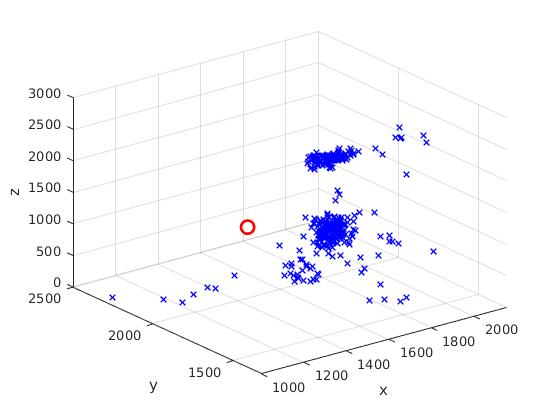
\includegraphics[width=\textwidth]{results/config1}
            \caption{Plot of Config 1}
        \end{subfigure}
        ~ %add desired spacing between images, e. g. ~, \quad, \qquad, \hfill etc.
          %(or a blank line to force the subfigure onto a new line)
        \begin{subfigure}[b]{0.49\textwidth}
            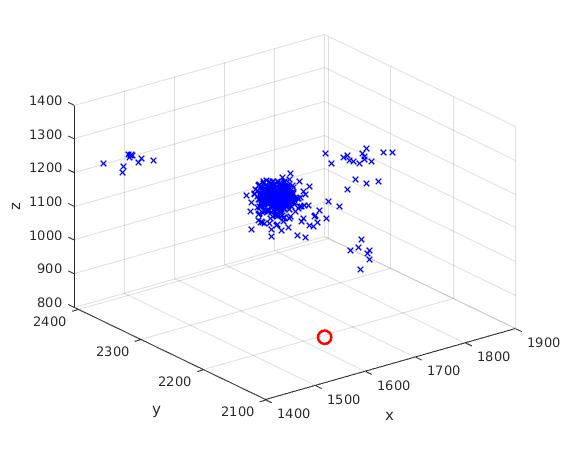
\includegraphics[width=\textwidth]{results/config6}
            \caption{Plot of Config 6}
        \end{subfigure}

        \begin{subfigure}[b]{\textwidth}
            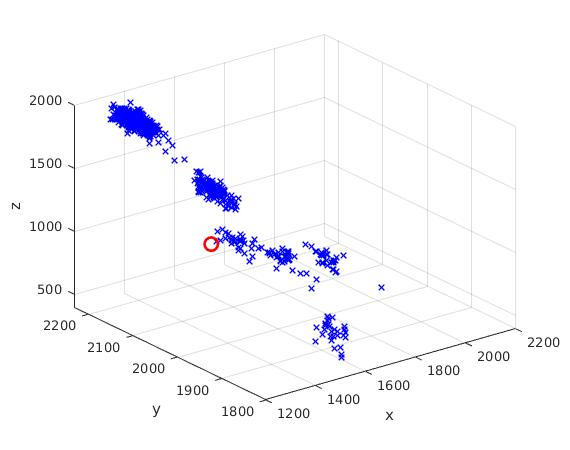
\includegraphics[width=\textwidth]{results/config11}
            \caption{Plot of Config 12}
        \end{subfigure}
        \caption{Sample plots of several anchor configurations.}
        \label{fig:config}
    \end{figure}

%TODO: Insert the pics I took of the anchors here.
Intro to the basic concept, highlight Pietra's paper and how I am using that to phrase and determine the best location
Show pics, diagrams and initial table of results?
